\chapter{Evaluation}
\label{chapter:evaluation}

\section{Calibration quality}
For computing the camera calibration error, another tool from the same ROS Camera Calibration package is used.
It continuously outputs a reprojection $\mathsf{RMS}$ (Root Mean Squared), which is defined as
\begin{equation}
    \mathsf{RMS}(x) = \sqrt{\frac{\sum_{i=1}^{N}{(x_i - \hat{x}_i)^2}}{N}}
\end{equation}
where $x$ is one measured data sample from the experiment, $\hat{x}$ is a ground-truth data, and $N$ is a sample size.
After launching this tool, we were moving a pattern in front of each camera to collect some data and analyse it.
The reprojection error varies depending on the pose of the chessboard, but in general is quite stable, see \autoref{tab:camcalib_eval}.

\begin{table}[ht]
    \begin{center}
      \begin{tabular}{ ll l l }
      \hline
      && Left camera & Right camera \\ \hline
      mean of RMS reprojection error & [px] & 0.06323214286 & 0.05357391304 \\
      variance of RMS reprojection error & [px] & 0.00001159968 & 0.00002222914 \\
      \end{tabular}
    \end{center}
    \caption{RMS reprojection error of the ROS Camera Calibration results.}
    \label{tab:camcalib_eval}
\end{table}

\section{Triangulation quality}
Two experiments were concluded to measure the triangulation quality.
The same pattern with visible key points in a featureless environment was used \autoref{fig:exp_process}.

\subsection{Experiment setup}
\label{sec:eval_setup}

\begin{figure}[ht]
    \centering
    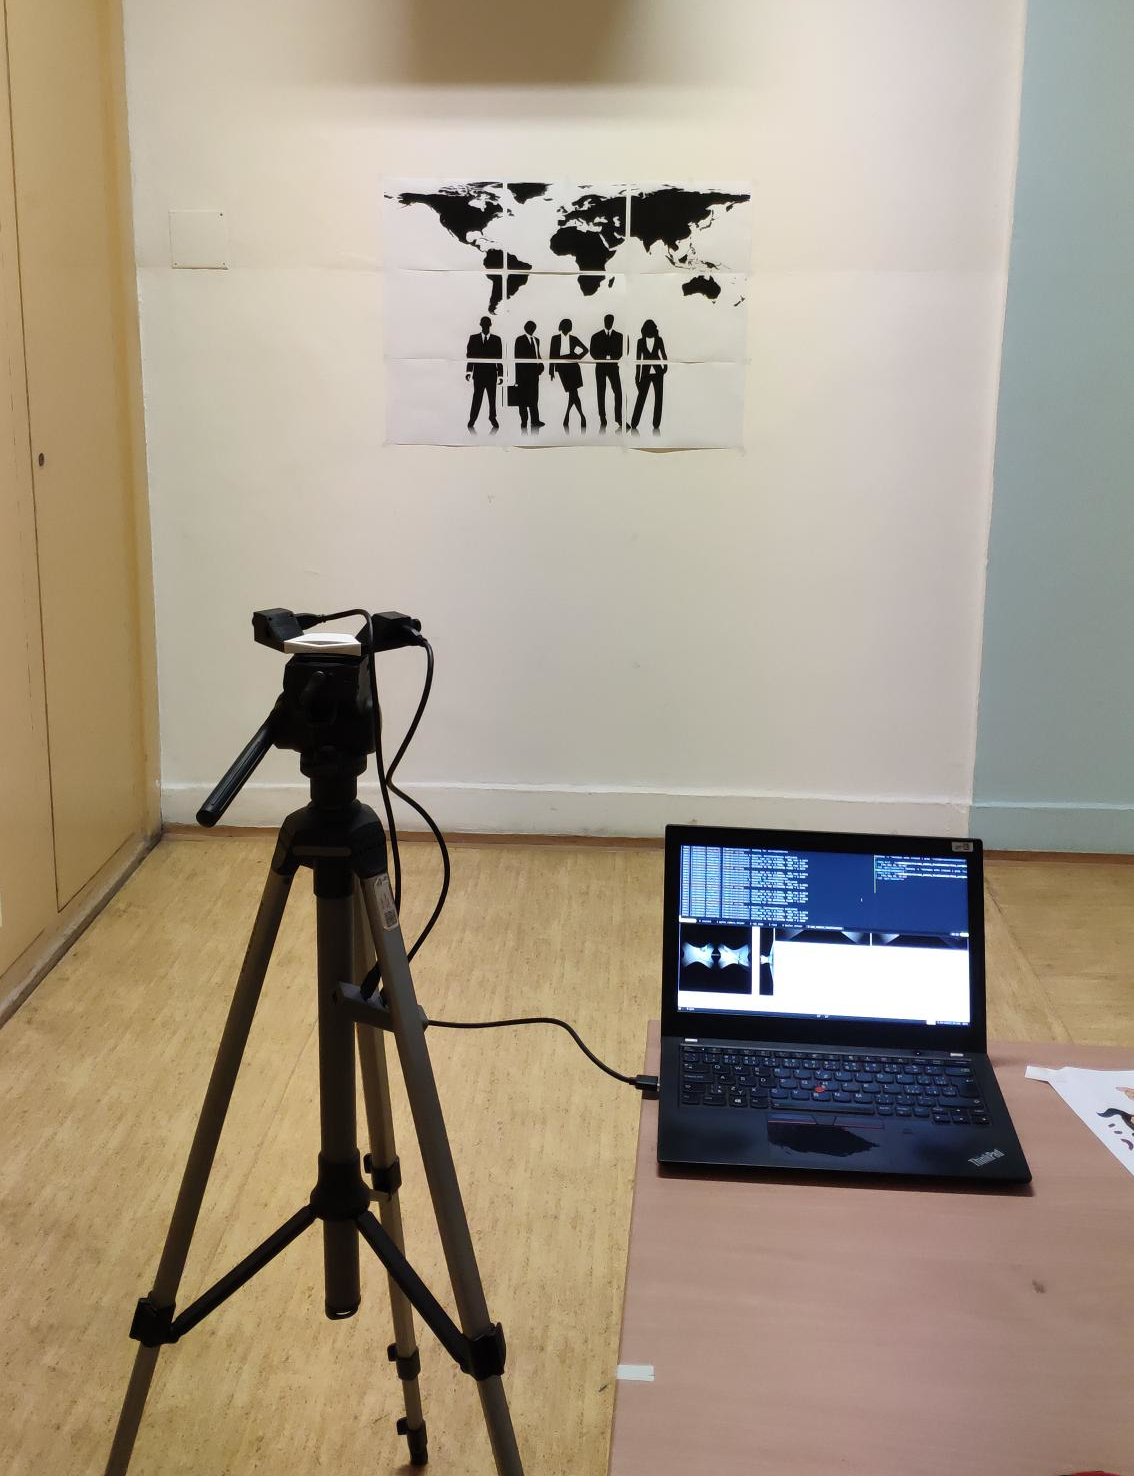
\includegraphics[width=0.6\textwidth]{graphics/experiment_setup.png}
    \caption[The setup for experiments]{The setup for experiments. 
    The designed prototype is located on a tripod, at distance $d$ from the plane $\Omega$ with visual features.
    The with y-z plane of the cameras' common coordinate frame is parallel with $\Omega$. 
    A set of 9 A4 papers with features was used to make $\Omega$ distinguishable.}
    \label{fig:exp_process}
\end{figure}

\begin{figure}[ht]
  \centering
  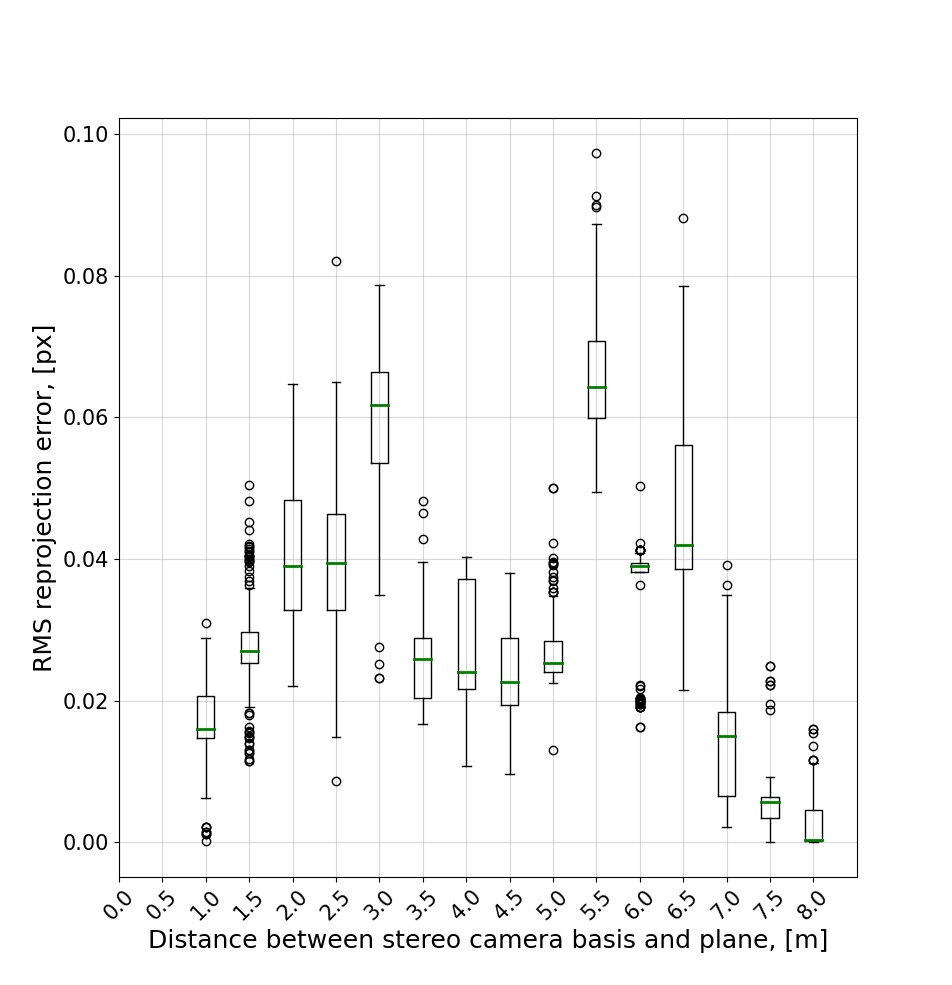
\includegraphics[width=0.5\textwidth]{graphics/experiment_1_repro_error.png}
  \caption[Stereo setup RMS reprojection error.]{Stereo pair setup RMS reprojection error. Red line represents the trend of the sample.}
  \label{fig:exp_1_repro}
\end{figure}

\begin{figure}[ht]
  \begin{subfigure}[ht]{0.49\textwidth}
    \centering
    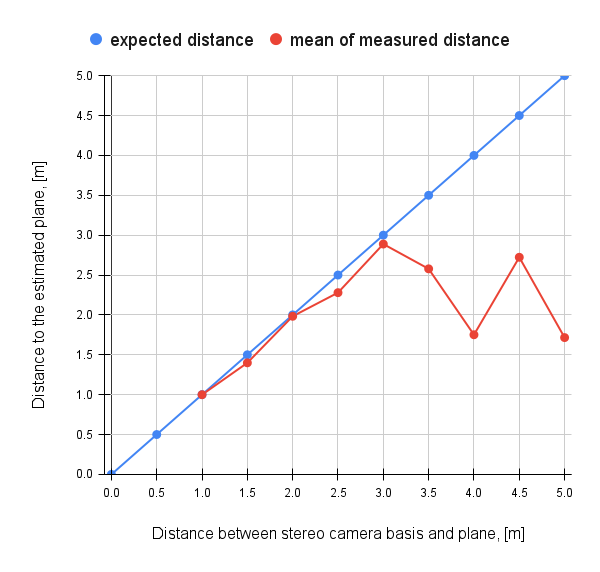
\includegraphics[width=\textwidth]{graphics/experiment_1_chart_planedist.png}
    \caption[Distance to the estimated plane]{Distance $d$ from the stereo camera to $\Omega$.
    Blue line represents the expected distance, and red line represents $d'$, computed as mean of $n$ estimated distances.}
    \label{fig:exp_1_chart_dists}
  \end{subfigure}
  \hfill
  \begin{subfigure}[ht]{0.49\textwidth}
    \centering
    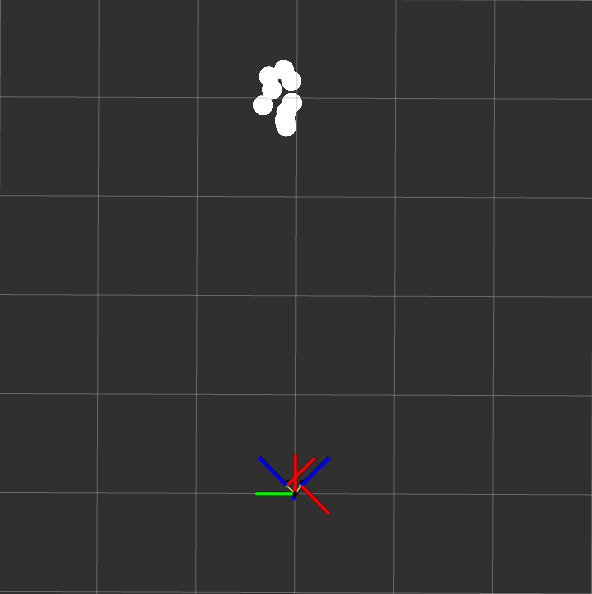
\includegraphics[width=\textwidth]{graphics/experiment_1_4m.png}
    \caption[Top view of the experiment.]{Top view of the experiment. 
    The grid's cell size is $1$m$\times$$1$m.
    The colored axes represent the stereo pair's coordinate system.
    Red color stands for $X$ axis, green for $Y$ and blue for $Z$.
    The basis aligned with the grid represents the stereo camera basis, $X$ axis towords the point cloud.
    The point cloud (white dots) represents the 3D points reconstructed from feature points seen by both cameras.}
    \label{fig:exp_1_topview}
  \end{subfigure}
  \caption{Results from the first experiment: distance to the estimated plane.}
  \label{fig:exp_1_exp}
\end{figure}

\begin{figure}[ht]
    \centering
    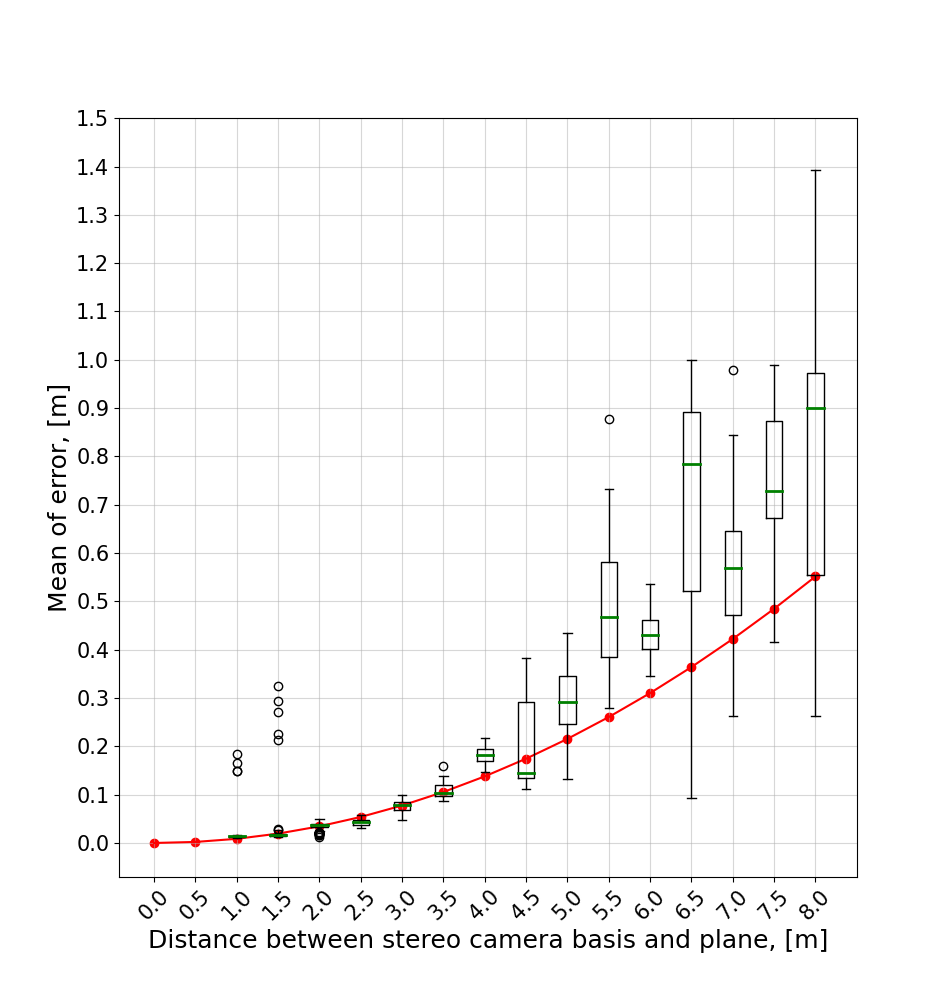
\includegraphics[width=\textwidth]{graphics/experiment_2_general.png}
  \caption[The second experiment results.]{The second experiment results. Red line represents the theoretical error for the given setup.
  Green lines represents the median for each $n$ measurements at a distance $d$. Box is drown from the first quartile to the third quartile.
  The whiskers go from each quartile to the minimum and maximum.
  Points represents outliers.}
  \label{fig:exp_2_general}
\end{figure}

The reprojection error is not a good metric to evaluate the triangulation performance because, with the distance increasing, the frature points are closer together, and the reprojection error decreases (see \autoref{fig:exp_1_repro}).
To measure the quality of distance estimation, a different approach was chosen.
A pattern with multiple features was attached to a white wall in a corridor within a featureless environment.
The camera prototype on a tripod was located at a fixed distance from the wall and was set up so that its $y-z$ plane was parallel to the wall as in \autoref{fig:exp_process}.
Based on this, we assume that the ground-truth position of all observed 3D points lies on a plane whose orientation and distance from the coordinate frame's origin are known.

Let us define the wall plane as $\Omega$, the distance from the origin of the stereo pair's common frame to the wall as $d$, an estimated plane as $\Omega'$ and an estimated distance to the plane as $d'$.
The number of timestamps for each experiment is $n$, and $i$ is a timestamp index, $i \in \{1 \dots n\}$.

The ground-truth distance was measured with the measuring tape, and the tripod was placed on a distance $d$ from the wall. 
Then $n$ measurements were made, and obtained data were collected and saved to post-process them separately, analysy and obtain plots.

The main goal of experiments is to measure the precision of triangulation and compare it with the theoretical error, introduced in \cite{cv_theoretical_error} as a function of the distance based on the geometrical and optical parameters of the setup.
The theoretical error is defined as
\begin{equation}
    e_Z = \frac{Z^2 \delta}{bf},
\end{equation}
where $Z$ is the real distance in, $\delta$ is a disparity error (error for keypoints matching, here - maximum possible distance to the corresponding epipolar error is used), $f$ is a focal length and $b = \lVert \vec{b} \rVert$ (see \autoref{fig:sch_stereo}).
To compute the theoretical error for the current prototype, the following data was used: $\delta=1$px, $f=38$mm and $b=14.5$mm.

\subsection{Distance to an estimated plane}
\label{sec:exp1}
For each set of 3D points corresponding to a specific distance $d$, the plane is estimated using RANSAC to filter outliers (an implementation from PCL was used).
The absolute difference between the distance from the camera to the computed plane and the distance from the camera to the wall plane is taken as the error.

The distance $d$ for this experiment was from $1$m to $5$m with a step of $0.5$m.
The result of this experiment is shown in \autoref{fig:exp_1_chart_dists}.
According to the figure, the distance deviates significantly after $3.5$m.
In \autoref{fig:exp_1_topview} the topview of the experiment is shown for $d=4$m.
It can be seen that the plane can not be estimated correctly at this distance because of a small error for each triangulated point.

\subsection{Distance to a predefined plane}
\label{sec:exp2}
With increasing the distance $d$, feature points become less distinguishable due to the limited resolution of the camera.
In \autoref{fig:exp_process}, the estimated plane $\Omega$ is inaccurate from a certain distance because of high noise in the $X$ direction of the points and low spread of the points in the $Y-Z$ direction (see \autoref{fig:exp_1_topview}), but still the points are close to the actual plane $\Omega$.
That is why the second experiment was constructed.

The experiment was done using the same setup as described in \autoref{sec:eval_setup}. 
The difference is that $\Omega'$ is not estimated using the least squares RANSAC method to fit the plane to the points, but as the plane parallel to $\Omega$ on a distance $e'_i$, that is defined as
\begin{equation}    
    e'_i = \frac{1}{k} \sum_{j=0}^{k}{|p'_j|},
\end{equation}
where $k$ is the number of keypoints detected at a timestamp $t_i$, and $p'_j$ is the distance from point $\vec{p}'_j$ to $\Omega$.

% In \autoref{fig:exp_2_general} the red line represents the theoretical error for the proposed setup.

The ground-truth distance $d$ for the current experiment was from $1$m to $8$m as the maximum distance at which key points can be detected (empirically found) with the step of $0.5$m.
The result of the second experiment is shown in \autoref{fig:exp_2_general}, where the received data follows the theoretical up to $4.0$ meters with a small deviation, and after that, it is also follows the pattern but with the bigger variance.
One of the possible problems here could be that the theoretical error does not include the error from the feature detector and matcher.
The second one is that there is an error in camera calibration and fixed focal length (cameras were calibrated on a small distance up to $3$m), so detected patterns on a bigger distances are blurred and less detectable. 

\section{Rate testing}
\begin{table}[ht]
    \begin{center}
      \begin{tabular}{ll}
      \hline
        Parameter & Value \\
        Minimal delay &  0.042s \\
        Maximal delay &  0.196s \\
        Average rate & 10.607Hz \\ 
      \end{tabular}
    \end{center}
    \caption{Measured data delay and rate of the proposed system.}
    \label{tab:eval_freq}
\end{table}

To ensure that obstacles can be detected, not only triangulation quality is important, but also the rate at which the MAV can receive the data from the obstacle avoidance module and the delay of the data.
The data rate, maximal and minimal delays for 5min are shown in \autoref{tab:eval_freq}.
 
\section{Experiments summary}
The quality of the distance estimation to obstacles was demonstrated in the two experiments.
The first experiment, described in \autoref{sec:exp1}, shows that the precision of the proposed method is relatively high for distances up to 3m, and the second experiment, described in \autoref{sec:exp2} provided further insight into the statistics of the error over longer distances. 
The estimated distance error on $3$m is less than $3\%$.
The maximum distance at which 3D points could be reliably estimated is $8$m with an error of up to $1$m.
On further distances, feature points can not be reliably detected anymore due to the camera resolution and focal length (cameras were calibrated on distances up to $2$m).
The proposed solution works with an average frequency of $10$Hz.
